\chapter{Introduction}
\label{introduction_chap}
The Weather Research and Forecasting (WRF) model is
a numerical weather prediction (NWP) and atmospheric simulation 
system designed for both 
research and operational applications.  WRF is supported 
as a common tool for the university/research and operational 
communities to promote closer ties between them and to 
address the needs of both.  The development of WRF has been a 
multi-agency effort to build a next-generation mesoscale forecast model 
and data assimilation system to advance the understanding and prediction 
of mesoscale weather and accelerate the transfer of research 
advances into operations.  The WRF effort has been a collaborative one 
among the National Center for Atmospheric Research's (NCAR) 
Mesoscale and Microscale Meteorology (MMM) Division, the 
National Oceanic and Atmospheric Administration's 
(NOAA) National Centers for Environmental Prediction (NCEP) and 
Earth System Research Laboratory (ESRL), the Department of Defense's 
Air Force Weather Agency (AFWA) and Naval Research Laboratory (NRL), 
the Center for Analysis and Prediction of Storms (CAPS) at the University 
of Oklahoma, and the Federal Aviation Administration (FAA), 
with the participation of university scientists. 

WRF reflects flexible, state-of-the-art, portable code that is 
efficient in computing environments ranging from massively-parallel
supercomputers to laptops. 
Its modular, single-source code can be configured for both 
research and operational applications.  Its spectrum of physics
and dynamics options reflects the experience and input of the 
broad scientific community.  Its WRF-Var variational data assimilation 
system can ingest a host of observation types in pursuit of 
optimal initial conditions, while its WRF-Chem  
model provides a capability for air chemistry modeling.

WRF is maintained and 
supported as a community model to facilitate wide use internationally, 
for research, operations, and teaching.
It is suitable for a broad span of applications across 
scales ranging from large-eddy to global simulations.  Such applications 
include real-time NWP, data assimilation 
development and studies, parameterized-physics research, regional 
climate simulations, air quality modeling, atmosphere-ocean coupling, and 
idealized simulations.  As of this writing, 
the number of registered WRF users exceeds 6000, and WRF is in 
operational and research use around the world.

The principal components of the WRF system are depicted in Figure 1.1. 
The WRF Software Framework (WSF) provides the infrastructure 
that accommodates the dynamics solvers, physics packages 
that interface with the solvers, programs for initialization,   
WRF-Var, and WRF-Chem.  There are two dynamics solvers in the WSF: the 
Advanced Research WRF (ARW) solver (originally referred to
as the Eulerian mass or $``$em" solver) developed primarily at NCAR, and
the NMM (Nonhydrostatic Mesoscale Model) solver developed at NCEP.
Community support for the former is provided by the MMM Division of NCAR 
and that for the latter is provided by the Developmental Testbed Center (DTC).


%
% Figure 1.1
%
\begin{figure}
  \centering
  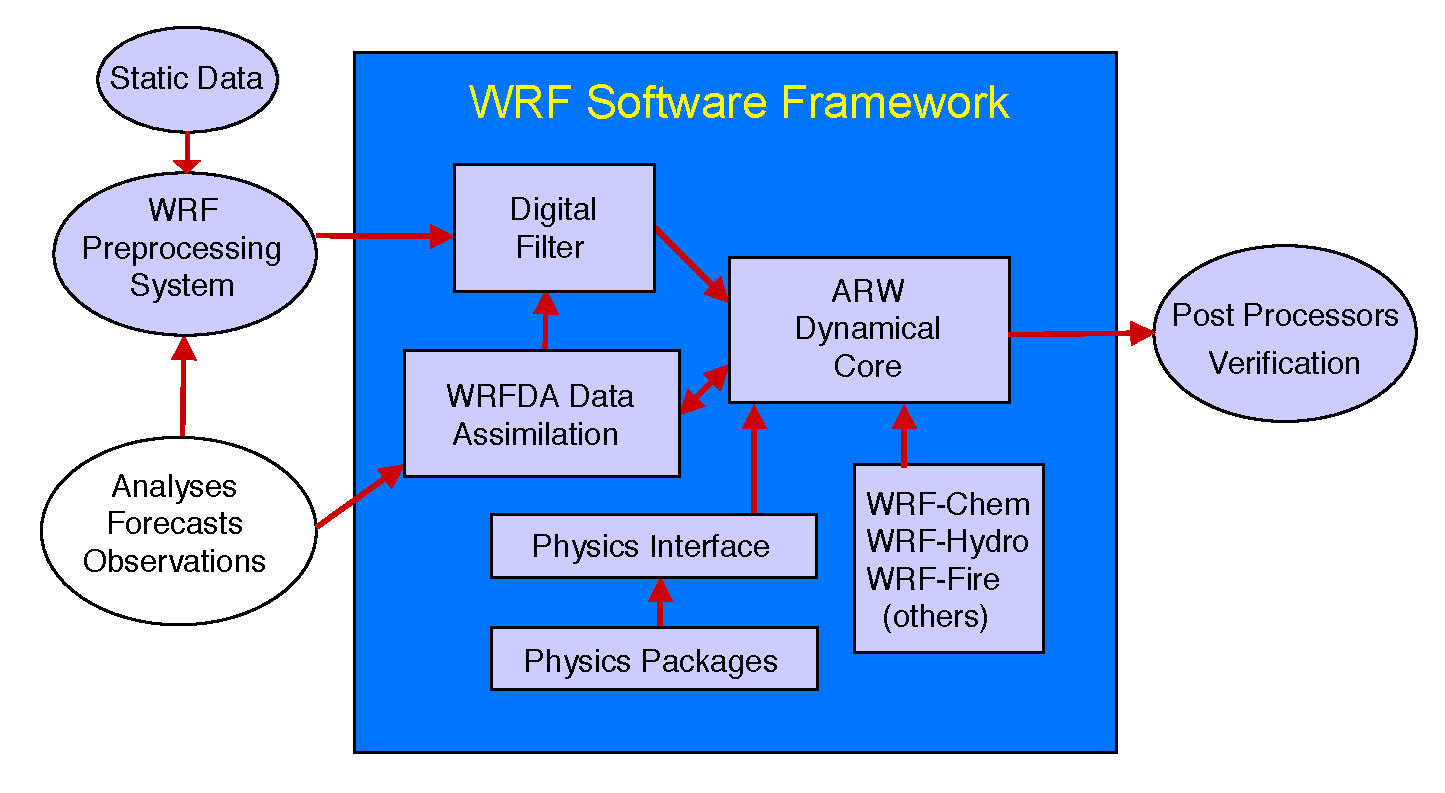
\includegraphics[width=6.5in]{figures/component.pdf}
  \caption{\label{figure:1}WRF system components.}
\end{figure}

\section {Advanced Research WRF}

The ARW is the ARW dynamics solver together with other
components of the WRF system compatible with that solver and 
used in producing a simulation.  Thus, it is a subset of 
the WRF modeling system that, in addition to the ARW solver, 
encompasses physics schemes, numerics/dynamics options, 
initialization routines, and a data assimilation package (WRF-Var).  
The ARW solver shares the WSF with the NMM solver and all other 
WRF components within the framework.  Physics packages are 
largely shared by both the ARW and NMM solvers, although specific 
compatibility varies with the schemes considered.  
The association of a component of the WRF system with 
the ARW subset does not preclude it from being a
component of WRF configurations involving the NMM solver.  
The following section highlights the major features of the 
ARW, Version 3, and reflects elements of WRF Version 3, 
which was first released in April 2008.

This technical note focuses on the scientific and algorithmic 
approaches in the ARW, including the solver, physics options,
initialization capabilities, boundary conditions, and grid-nesting techniques.  
The WSF provides the software infrastructure.  
WRF-Var, a component of the broader WRF system, was  
adapted from MM5 3DVAR \citep{barker04} and is encompassed within the ARW.
While WRF-Chem is part of the ARW, Version 3, it is described 
outside of this technical note.  Those seeking details on 
WRF-Chem may consult \citet{Grelletal05} and 
http://ruc.fsl.noaa.gov/wrf/WG11/status.htm . 
For those seeking information on running the ARW system, 
the {\wrf} User's Guide \citep{wang08} 
has the details on its operation. 

\section {Major Features of the ARW System, Version 3}

\vskip 12pt
{\noindent\bf ARW Solver}
\vskip 12pt

\begin{description}
\setlength{\itemsep}{-5pt}
\item{$\bullet$} {\em Equations:}
Fully compressible, Euler nonhydrostatic with 
a run-time hydrostatic option available. Conservative for scalar variables.
%
\item{$\bullet$} {\em Prognostic Variables:}
Velocity components $u$ and $v$ in Cartesian coordinate, vertical velocity $w$, 
perturbation potential temperature, perturbation geopotential, 
and perturbation surface pressure of dry air.
Optionally, turbulent kinetic energy and any number of scalars
such as water vapor mixing ratio, rain/snow mixing ratio,
cloud water/ice mixing ratio, and chemical species and tracers.
%
\item{$\bullet$} {\em Vertical Coordinate:}
Terrain-following, dry hydrostatic-pressure, with vertical grid stretching permitted.
Top of the model is a constant pressure surface.
%
\item{$\bullet$} {\em Horizontal Grid:}
Arakawa C-grid staggering. 
%
\item{$\bullet$} {\em Time Integration:}
Time-split integration using a 2nd- or 3rd-order Runge-Kutta scheme with
smaller time step for acoustic and gravity-wave modes. 
Variable time step capability.
%
\item{$\bullet$} {\em Spatial Discretization:}
2nd- to 6th-order advection options in horizontal and vertical.
%
\item{$\bullet$} {\em Turbulent Mixing and Model Filters:} Sub-grid scale
turbulence formulation in both coordinate and physical space.
Divergence damping, external-mode filtering, vertically implicit
acoustic step off-centering. Explicit filter option.
%
\item{$\bullet$} {\em Initial Conditions:}
Three dimensional for real-data, and one-, two- and 
three-dimensional for idealized data. 
Digital filtering initialization (DFI) capability 
available (real-data cases).
%
\item{$\bullet$} {\em Lateral Boundary Conditions:} 
Periodic, open, symmetric, and specified options available.
%
\item{$\bullet$} {\em Top Boundary Conditions:} 
Gravity wave absorbing (diffusion, Rayleigh damping, or implicit 
Rayleigh damping for vertical velocity).  
Constant pressure level at top boundary along a material surface. 
Rigid lid option.
%
\item{$\bullet$} {\em Bottom Boundary Conditions:} 
Physical or free-slip.
%
\item{$\bullet$} {\em Earth's Rotation:}
Full Coriolis terms included.
%
\item{$\bullet$} {\em Mapping to Sphere:} 
Four map projections are supported for real-data simulation: 
polar stereographic, Lambert conformal, Mercator, and 
latitude-longitude (allowing rotated pole). 
Curvature terms included.
%
\item{$\bullet$} {\em Nesting:} 
One-way interactive, two-way interactive, and moving nests.
Multiple levels and integer ratios.
%
\item{$\bullet$} {\em Nudging:}
Grid (analysis) and observation nudging capabilities available. 
%
\item{$\bullet$} {\em Global Grid:}
Global simulation capability using polar Fourier filter and 
periodic east-west conditions. 
\end{description}

\newpage
\vskip 12pt
{\noindent\bf Model Physics}
\vskip 12pt

\begin{description}
\setlength{\itemsep}{-5pt}
\item{$\bullet$} {\em Microphysics:} Schemes ranging from simplified
physics suitable for idealized studies to sophisticated mixed-phase
physics suitable for process studies and NWP.
%
\item{$\bullet$} {\em Cumulus parameterizations:}
Adjustment and mass-flux schemes for mesoscale modeling.
%
\item{$\bullet$} {\em Surface physics:}
Multi-layer land surface models ranging from a simple thermal model to full
vegetation and soil moisture models, including snow cover and sea ice.
%
\item{$\bullet$} {\em Planetary boundary layer physics:}
Turbulent kinetic energy prediction or non-local $K$ schemes.
%
\item{$\bullet$} {\em Atmospheric radiation physics:} 
Longwave and shortwave schemes with multiple spectral bands and a 
simple shortwave scheme suitable for climate and weather applications.  
Cloud effects and surface fluxes are included.
\end{description}

\vskip 12pt
{\noindent\bf WRF-Var System}
\vskip 12pt

\begin{description}
\setlength{\itemsep}{-5pt}
\item{$\bullet$} WRF-Var merged into WRF software framework.
%
\item{$\bullet$} Incremental formulation of the model-space cost function.
%
\item{$\bullet$} Quasi-Newton or conjugate gradient minimization algorithms.
%
\item{$\bullet$} Analysis increments on unstaggered Arakawa-A grid.
%
\item{$\bullet$} Representation of the horizontal component of background error ${\bf B}$ via
recursive filters (regional) or power spectra (global). The
vertical component is applied through projection onto climatologically-averaged 
eigenvectors of vertical error. Horizontal/vertical errors are
non-separable (horizontal scales vary with vertical eigenvector).
%
\item{$\bullet$}  Background cost function ($J_b$) preconditioning 
via a control variable transform ${\rm U}$ defined as ${\bf B}={\rm U} {\rm U}^T$.
%
\item{$\bullet$} Flexible choice of background error model and control variables.
%
\item{$\bullet$} Climatological background error covariances estimated via either the
NMC-method of averaged forecast differences or suitably averaged
ensemble perturbations.
%
\item{$\bullet$} Unified 3D-Var (4D-Var under development), global 
and regional, multi-model capability.
%
\end{description}

\vskip 12pt
{\noindent\bf WRF-Chem}
\vskip 12pt

\begin{description}
\setlength{\itemsep}{-5pt}
\item{$\bullet$} Online (or ``inline'') model, in which the model is consistent
with all conservative transport done by the meteorology model. 
%
\item{$\bullet$} Dry deposition, coupled with the soil/vegetation scheme.
%
\item{$\bullet$} Aqueous phase chemistry coupled to some of the microphysics and aerosol schemes.
%
\item{$\bullet$} Three choices for biogenic emissions:
No biogenic emissions; Online calculation of biogenic emissions; Online modification 
of user specified biogenic emissions (e.g., EPA Biogenic Emissions Inventory System (BEIS)).
%
\item{$\bullet$} Two choices for anthropogenic emissions:
No anthropogenic emissions and user-specified anthropogenic emissions.
%
\item{$\bullet$} Two choices for gas-phase chemical reaction calculations:
RADM2 chemical mechanism and CBM-Z mechanism.
%
\item{$\bullet$} Several choices for gas-phase chemical reaction calculations 
through the use of the Kinetic Pre-Processor (KPP). 
%
\item{$\bullet$} Three choices for photolysis schemes:
Madronich scheme coupled with hydrometeors, aerosols, and convective parameterizations;
Fast-J Photolysis scheme coupled with hydrometeors, aerosols, and convective parameterizations;
FTUV scheme scheme coupled with hydrometeors, aerosols, and convective parameterizations.
%
\item{$\bullet$} Choices for aerosol schemes:
The Modal Aerosol Dynamics Model for Europe (MADE/SORGAM);
Model for Simulating Aerosol Interactions and Chemistry (MOSAIC); and 
The GOCART aerosol model (experimental). 
%
\item{$\bullet$} A tracer transport option in which the chemical mechanism, 
deposition, etc., has been turned off. 
\end{description}

\vskip 12pt
{\noindent\bf WRF Software Framework}
\vskip 12pt

\begin{description}
\setlength{\itemsep}{-5pt}
\item{$\bullet$} Highly modular, single-source code for maintainability.
%
\item{$\bullet$} Two-level domain decomposition for parallel and 
shared-memory generality.
%
\item{$\bullet$} Portable across a range of available computing platforms.
%
\item{$\bullet$} Support for multiple dynamics solvers and physics modules.
%
\item{$\bullet$}
Separation of scientific codes from parallelization and other 
architecture-specific issues.
%
\item{$\bullet$}
Input/Output Application Program Interface (API) enabling various external
packages to be installed with WRF, thus allowing WRF
to easily support various data formats.
%
\item{$\bullet$}
Efficient execution on a range of computing platforms
(distributed and shared memory, vector
and scalar types). Support for accelerators (e.g., GPUs).
%
\item{$\bullet$}
Use of Earth System Modeling Framework (ESMF) and interoperable as an ESMF
component.
%
\item{$\bullet$}
Model coupling API enabling WRF to be coupled with other models such as
ocean, and land models using ESMF, MCT, or MCEL.
\end{description}
